\chapter{基于邻接链表的图的实现}\label{chapter:4}

\section{实验目的}\label{sec:test41}
通过实验达到
\begin{itemize}
    \item 加深对图的概念、基本运算的理解
    \item 熟练掌握图的逻辑结构与物理结构的关系
    \item 以邻接链表作为物理结构,熟练掌握图基本运算的实现。
\end{itemize}

\subsection{对图对理解}
通过本次实验,我对\textbf{图}又有了更多的了解,由于图的结构比较复杂,任意两个节点之间都可能存在联系,因此无法以数据元素存储区中的物理位置来表示元素之间的关系,即图没有顺序映像的存储结构,但可以借助数组数据类型表示元素之间的关系。~\cite{严蔚敏2002数据结构}
\subsection{对邻接链表的理解}
\textbf{邻接链表}是图的一种链式存储结构。在邻接链表中,对图中每个顶点建立一个单链表,第$i$个单链表中的节点表示依附于顶点$v_{i}$的边(对有向图是以顶点$v_{i}$为尾的弧)。每个结点由三个域组成,其中邻接点域指示域顶点$v_{i}$邻接的点在图中的位置,链域指示下一条边或弧的结点,数据域存储和边和或弧相关的信息,如权值等。每个链表上附设有头指针。~\cite{严蔚敏2002数据结构}
\newline
\subsection{对基本运算的理解与实现}
总的来说,图的基本运算较简单,主要的难点在创建(\texttt{create})插入 (\texttt{insert})节点与删除 (\texttt{delete})节点和边。
因为需要对图的邻接链表进行改变,并且对相应的节点进行相应的插入和删除操作
同时要分配新的内存并创建新的节点。
如果操作不当,或者没有对用户的输入进行校验,插入或删除出错。
\subsection{单元测试}
通过编写完整的单元测试,将可能出现的错误都考虑清楚,尽量实现测试覆盖率达到100\%。
从而保证了程序在正确情况和极端情况下都能正常运行。

% ------------------------------------------------------------

\section{实验内容}\label{sec:test42}
    实验内容主要分为一下三个部分:
\begin{enumerate}
    \item 问题描述
    \item 系统设计
    \item 系统实现
\end{enumerate}
\section{问题描述}
\subsection{图的定义}
\begin{definition}\label{def:binarytree5}
    图 (\emph{Graph})中的数据原属通常称为顶点,$V$是顶点的有穷非空集合,$VR$是两个顶点之间关系的集合。若$(v,w)\in
    VR$则表示从$v$到$w$有一条弧,且称$v$为弧尾 (Tail),称$w$为弧头 (Head),此时的图称为有向图,若$VR$是对称的,则称此时的图为无向图。
\end{definition}
其中:
\begin{itemize}
    \item 数据节点可以为任意类型,但同一图中节点类型必须相同。
    \item 数据节点的个数$n$定义为图的大小,图里没有一个节点时称为空图。
    \item 具有$n(n-1)$条弧的图称为有向完全图。
    \item 有很少条边或弧的图称为稀疏图,反之则称为稠密图。
\end{itemize}

\subsection{图相关术语}

根据图中顶点间是否有路径,可以将图分为连通图与非连通图。

\begin{definition}
    在无向图中,如果从顶点$v$到顶点$v'$有路径,则称$v$和$v'$是连通的。如果对于图中任意两个顶点$v_i,\,v_j\in V,v_i,\,v_j$都是连通的,则称$G$是连通图。
\end{definition}

而由此我们也可以得到连通分量的概念。

\begin{definition}
    所谓连通分量,字的事无向图中的极大连通子图。
\end{definition}

有了连通分量的概念,我们可以得到生成树的概念。

\begin{definition}
    一个连通图的生成树是一个极小连通子图,她含有图中全部节点,但只有足以构成一棵树但$n-1$条边。
\end{definition}

邻接链表的存储特点是:只要确定了\emph{一个顶点},所有与之相连的顶点就可以很简单的通过遍历链表来获得。

\subsection{实验需要完成的基本操作}
\begin{enumerate}
\item 创建图:\texttt{CreateGraph (G)},\newline \textbf{\emph{初始条件}}是图G不存在 。\newline \textbf{\emph{操作结果}}是构造一个空的图。
\item 销毁图:\texttt{DestroyGraph (G)},\newline \textbf{\emph{初始条件}}是图G已存在。\newline \textbf{\emph{操作结果}}是销毁图G。
\item 清空图:\texttt{ClearGraph (G)},\newline \textbf{\emph{初始条件}}是图G已存在 。\newline \textbf{\emph{操作结果}}是将G重置为空图。
\item 查找节点:\texttt{LocateVex (G,e)},\newline \textbf{\emph{初始条件}}是图已存在 。\newline
    \textbf{\emph{操作结果}}返回查找到的结点指针,如无关键字为e的结点,返回NULL。
\item 节点赋值:\texttt{AssginVex (G,e,value)},\newline \textbf{\emph{初始条件}}是图G已存在 。\newline \textbf{\emph{操作结果}}是关键字为e的结点赋值为value。
\item 插入节点:\texttt{InsertVex (G,e,c)},\newline \textbf{\emph{初始条件}}是图G已存在且非空。\newline \textbf{\emph{操作结果}}插入结点c到G中,作为关键字为e的结点
\item 删除节点:\texttt{DeleteVex (G,i,e)},\newline \textbf{\emph{初始条件}}是图G已存在且非空。\newline
    \textbf{\emph{操作结果}}:是删除G中关键字为e的结点,同时删除所有与之相连的边。
\item 插入弧:\texttt{InsertArc  (G,src,dst)},\newline \textbf{\emph{初始条件}}是图G已存在且非空,且src dst均存在。\newline
    \textbf{\emph{操作结果}}从src插入一条到dst的弧。
\item 删除弧:\texttt{DeleteArc  (G,i,e)},\newline \textbf{\emph{初始条件}}是图G已存在且非空。\newline
    \textbf{\emph{操作结果}}:是删除G中关键字为e的弧,但保留弧所连接的结点;
\item 深度优先搜索:\texttt{DFS(G,visit ())},\newline \textbf{\emph{初始条件}}是图G已存在,\newline \textbf{\emph{操作结果}}根据深度优先对G的每个数据节点调用函数visit ()。
\item 广度优先搜索:\texttt{BFS(G,visit ())},\newline \textbf{\emph{初始条件}}是图G已存在,\newline \textbf{\emph{操作结果}}根据广度优先对G的每个数据节点调用函数visit ()。
\item 第一个邻接点:\texttt{FirstAdjVex(G,index)},\newline \textbf{\emph{初始条件}}是图G已存在,\newline
    \textbf{\emph{操作结果}}获得第index个结点的第一个邻接顶点。
\item 层级遍历:\texttt{NextAdjVex(G,Vindex,Aindex)},\newline \textbf{\emph{初始条件}}是图G已存在,\newline
    \textbf{\emph{操作结果}}获得第Vindex个顶点第Aindex+1个邻接顶点。
\end{enumerate}

\section{系统设计}
\subsection{总体设计}
本系统采用\emph{邻接链表}作为图的物理结构,实现有向图的基本运算。
\par
系统开始运行的时候默认不使用文件中的数据,但是用户随时可以将文件中的数据导入到内存中,同时提供数据保存的功能。
\subsection{有关常量和类型定义}
采取\texttt{C++}中的模版类来使图支持所有类型的数据,
\par
对于程序中可能出现的错误,进行统一规定:
\begin{enumerate}
    \item 对于用户输入不正确导致的在错误的位置插入或者删除,统一抛出\texttt{range\_error}。
    \item 对于其他可能发生的错误,统一抛出\texttt{runtime\_error}。
\end{enumerate}
\subsubsection{函数设计}
头文件中的函数原型声明见\autoref{appendix:h4}
函数时间复杂度分析见\autoref{tab:timeandspace4}
\begin{table}[ht]
\centering
\caption{函数时间与空间复杂度分析}
\label{tab:timeandspace4}
\begin{tabular}{@{}ccccc@{}}
\toprule
编号                          & 名称  & 函数签名 & 时间复杂度 & 空间复杂度 \\ \toprule
    \multicolumn{1}{c|}{1}  & 创建图 & \texttt{ createGraph()} & $O(V+E)$ &  $O(V+E)$ \\
    \multicolumn{1}{c|}{2}  & 销毁图& \texttt{ destroyGraph()} & $O(V+E)$ &  $O(V+E)$ \\
    \multicolumn{1}{c|}{3}  & 清空图& \texttt{ clearGraph()} & $O(1)$ &  $O(1)$   \\
    \multicolumn{1}{c|}{4}  & 获得结点值& \texttt{ getVexValue()} & $O(V)$ &  $O(1)$     \\
    \multicolumn{1}{c|}{5}  & 第一个邻接点& \texttt{ firstAdjVex()} & $O(V)$ &  $O(1)$     \\
    \multicolumn{1}{c|}{6}  & 下一个邻接点& \texttt{ nextAdjVex()} & $O(V+E)$ &  $O(V+E)$      \\
    \multicolumn{1}{c|}{7}  & 查找节点 & \texttt{ locate()} & $O(V)$ &  $O(1)$   \\
    \multicolumn{1}{c|}{8}  & 插入节点 & \texttt{ insertVex()} & $O(V)$ &  $O(1)$    \\
    \multicolumn{1}{c|}{9}  & 插入弧 & \texttt{ insertArc()} & $O(V+E)$ &  $O(1)$     \\
    \multicolumn{1}{c|}{10}  & 删除节点 & \texttt{ deleteVex()} & $O(V+E)$ &  $O(1)$  \\
    \multicolumn{1}{c|}{11}  & 删除节点 & \texttt{ deleteArc()} & $O(V+E)$ &  $O(1)$  \\
    \multicolumn{1}{c|}{12}  & 深度优先搜索& \texttt{ bfs()}   & $O(V+E)$ & $O(V+E)$ \\
    \multicolumn{1}{c|}{13}  & 广度优先搜索& \texttt{ bfs()}   & $O(V+E)$ & $O(V+E)$ \\ \bottomrule
\end{tabular}
\end{table}
\subsubsection{算法设计}
\paragraph{创建算法}如\autoref{alg:create4}所示,时间复杂度为$O(V+E)$,空间复杂度为$O(1)$
\par
\begin{algorithm}[H]
    \SetAlgoLined
    \KwIn{Def}
    \KwOut{Graph}
    \If{Def is invalid}{throw error}
    let $G$ be an empty graph\;
    \For{v=firstVex of Def; v\leq lastVex of Def; v++}{
        G.insertVex(v)\;
    }
    \For{a=firstArc of Def; a\leq lastArc of Def; a++}{
        G.insertArc(a)\;
    }
    \caption{Create}\label{alg:create4}
\end{algorithm}
\paragraph{插入算法}如\autoref{alg:insert4}述,其时间复杂度为$O(V)$,空间复杂度为$O(1)$
\par
\begin{algorithm}[H]
    \SetAlgoLined
    \KwIn{elem}
    \KwOut{none}
    \If{index out of range}{ throw error}
    let v = a new Vex with value elem\;
    G.InsertVex(v)\;
\caption{InsertVex}\label{alg:insert4}
\end{algorithm}
\paragraph{删除结点算法}如\autoref{alg:delete44}所述,其时间复杂度为$O(V+E)$,空间复杂度为$O(1)$
\begin{algorithm}[th]
    \SetAlgoLined
    \KwIn{value}
    \KwOut{none}
    \For{v=first vex of G; v < G.VexNumber; v++}{
        \For{a=first arc of v; v<v.ArcNumber;a++}{
            \If{a.to == value}{delete a}
        }
        \If{G.at(v)==value}{delete v}
    }
\caption{DeleteVex}\label{alg:delete44}
\end{algorithm}
\paragraph{插入弧算法}如\autoref{alg:insertArc}所示,时间复杂度为$O(V+E)$,空间复杂度为$O(1)$
\par
\begin{algorithm}[H]
    \SetAlgoLined
    \KwIn{from, to, weight}
    \KwOut{none}
    \For{v=first vex of G; v< G.VexNumber; v++}{
        \If{v==to}{
            v.insertArc(to,weight)\;
        }
    }
    \caption{InsertArc}\label{alg:insertArc}
\end{algorithm}
\paragraph{删除弧算法}如\autoref{alg:delete4}所示,时间复杂度为$O(V+E)$,空间复杂度为$O(1)$
\par
\begin{algorithm}[H]
    \SetAlgoLined
    \KwIn{from,to}
    \KwOut{none}
    \For{v=first vex of G; v< G.VexNumber; v++}{
        \If{v==from}{
            \For{a=v.first arc; a<v.ArcNumber;a++}{
                \If{a==to}{
                    delete a\;
                }
            }
        }
    }
    \caption{DeleteArc}\label{alg:delete4}
\end{algorithm}
\section{系统实现}
\subsection{开发环境}
本次实验中使用的环境如下:
\begin{enumerate}
    \item 操作系统版本 Darwin X86\_64 Kernel Version 19.2.0
    \item 编译器及其版本 clang++ version 11.0.0 (Apple LLVM version 11.0.0)
    \item 自动编译工具 CMake version 3.16.1
    \item 编程环境 NeoVim
\end{enumerate}
\subsection{代码结构及源代码}
本次实验采取了模块化的编码方式,
\footnote{具体代码结构见\autoref{appendix:structure}}
将图的不同部分的功能放置在不同源文件中,
\footnote{源代码见\autoref{appendix:lab4},测试代码见\autoref{appendix:test4}}
分别编译后链接,提高了代码的可维护性和编译速度,同时也更加容易编写单元测试,保证代码的正确性。
\subsection{代码亮点}
\begin{enumerate}
        \item 所有的代码均采用\emph{Google
            C/C++}标准代码规范以及\emph{ISOC++}委员会所推荐的\emph{CPP Core Guidelines}代码规范,同时使用\texttt{clang-format}和\texttt{clang-tidy}对代码进行格式化和规范化,符合现代化C++的规范。
        \item 所有代码均尽可能采用更新的C++标准,以提高可维护性以及可读性。
        \item 采用智能指针\footnote{需要C++11及以上的编译器支持}(\texttt{unique\_ptr})进行资源管理,避免了手动管理内存所可能造成的内存泄露等问题。
        \item 所有函数及变量均采用\texttt{auto}关键字进行声明,避免了错误的类型声明以及隐式的类型转换。
        \item 采用C++的模板类(\texttt{template})来实现图,体现出了图中能存放任何类型的节点、但同一图中只能存放单一类型节点的特点。
        \item 采用\texttt{CMake}自动生成\texttt{Makefile},从而简化了构建过程,同时能够实现跨平台编译。
        \item 使用现代化的C++测试框架\texttt{Catch2},简化了测试流程。
        \item 采用TDD\footnote{Test Driven Development}的开发方式,在保证效率的情况下尽可能地提高测试覆盖度,使系统更健壮,更容易维护。
        \item 使用\texttt{Sanitize}与\texttt{Valgrind}对代码进行检测,发现可能存在的内存泄漏或未定义行为。
        \item 使用\texttt{gcov, lcov, llvm-cov gcov}等工具对单元测试的覆盖度进行检测,并生成相应的测试报告。
\end{enumerate}

\subsection{系统测试}
本系统使用了\textit{Catch2}\footnote{url: https://github.com/catchorg/Catch2}作为测试框架,
对所有源代码编写了\textbf{完善}的单元测试,可以做到所有边界情况和越界情况以及正常情况全部覆盖,
同时程序中的每一个分支也都进行测试,使得测试覆盖度基本达到100\%。
% Please add the following required packages to your document preamble:
\subsubsection{构造函数测试}
\textbf{输入:}\texttt{Def}变量,创建的图定义。
\par
\textbf{输出:}\texttt{std::vector<T> res},图深度优先搜索的结果。
\par
\textbf{预计结果:}深度优先搜索正确。
\begin{table}[h]
\centering
\caption{构造函数测试}
\begin{tabular}{@{}ccccc@{}}
\toprule
\multicolumn{1}{c}{测试类型}    & \multicolumn{1}{c}{测试输入} & \multicolumn{1}{c}{理论输出} & \multicolumn{1}{c}{实际输出} & \multicolumn{1}{c}{测试结果} \\ \midrule
\multicolumn{1}{c|}{正确性测试}  & 随机一棵图的Def&深度优先搜索&深度优先搜索&正确\\
\multicolumn{1}{c|}{正确性测试}  & 空(默认构造函数)&1&1&正确\\
\multicolumn{1}{c|}{错误处理测试} & 错误定义& std::underflow\_error& std::underflow\_error& 正确\\ \bottomrule
\end{tabular}
\label{tab:inittest4}
\end{table}

\subsubsection{判定空图函数测试}
\textbf{输入:}\texttt{graph}变量,一个图。
\par
\textbf{输出:}\texttt{graph.empty()},图是否为空。
\par
\textbf{预计结果:}对于空图,输出\texttt{true},否则输出\texttt{false}。
\begin{table}[h]
\centering
    \caption{\texttt{判定空图函数测试}}
\begin{tabular}{@{}ccccc@{}}
\toprule
\multicolumn{1}{c}{测试类型}    & \multicolumn{1}{c}{测试输入} & \multicolumn{1}{c}{理论输出} & \multicolumn{1}{c}{实际输出} & \multicolumn{1}{c}{测试结果} \\ \midrule
\multicolumn{1}{c|}{正确性测试}  & 空graph&true&true&正确\\
\multicolumn{1}{c|}{正确性测试}  & 非空graph&false&false&正确\\ \bottomrule
\end{tabular}
\label{tab:emptytest4}
\end{table}


\subsubsection{销毁图测试}
\textbf{输入:}无
\par
\textbf{输出:}无
\par
\textbf{预计结果:}图被销毁
\begin{table}[h]
\caption{销毁图测试}
\centering
\begin{tabular}{@{}ccccc@{}}
\toprule
\multicolumn{1}{c}{测试类型}    & \multicolumn{1}{c}{测试输入} & \multicolumn{1}{c}{理论输出} & \multicolumn{1}{c}{实际输出} & \multicolumn{1}{c}{测试结果} \\ \midrule
\multicolumn{1}{c|}{正确性测试}  & 无&图被销毁&图被销毁&正确\\ \bottomrule
\end{tabular}
\label{tab:destorytest4}
\end{table}


\subsubsection{清空图测试}
\textbf{输入:}无
\par
\textbf{输出:}无
\par
\textbf{预计结果:}图被清空
\begin{table}[h]
    \centering
    \caption{清空图测试}
    \begin{tabular}{@{}ccccc@{}}
        \toprule
        \multicolumn{1}{c}{测试类型}    & \multicolumn{1}{c}{测试输入} & \multicolumn{1}{c}{理论输出} & \multicolumn{1}{c}{实际输出} &
        \multicolumn{1}{c}{测试结果} \\ \midrule
        \multicolumn{1}{c|}{正确性测试}  &无 &图被清空&图被清空&正确\\ \bottomrule
    \end{tabular}
    \label{tab:cleartest4}
\end{table}


\subsubsection{求第一个邻接点测试}
\textbf{输入:}一个图,index
\par
\textbf{输出:}value,第一个邻接点的值
\par
\textbf{预计结果:}输出与实际值相等。
\begin{table}[h]
    \centering
    \caption{求第一个邻接点}
    \begin{tabular}{@{}ccccc@{}}
        \toprule
        \multicolumn{1}{c}{测试类型}    & \multicolumn{1}{c}{测试输入} & \multicolumn{1}{c}{理论输出} & \multicolumn{1}{c}{实际输出} &
        \multicolumn{1}{c}{测试结果} \\ \midrule
        \multicolumn{1}{c|}{正确性测试}  & 5&5&5&正确\\
        \multicolumn{1}{c|}{正确性测试}  & 空图&0&0&正确\\ \bottomrule
    \end{tabular}
    \label{tab:lengthtest4}
\end{table}


\subsubsection{查找节点测试}
\textbf{输入:}\texttt{key}变量,要获取节点的key。
\par
\textbf{输出:}\texttt{element},获得到的节点。
\par
\textbf{预计结果:}想要获取到的节点与实际获取的节点相等。
\begin{table}[h]
    \centering
    \caption{查找节点测试}
    \begin{tabular}{@{}ccccc@{}}
        \toprule
        \multicolumn{1}{c}{测试类型}    & \multicolumn{1}{c}{测试输入} & \multicolumn{1}{c}{理论输出} & \multicolumn{1}{c}{实际输出} &
        \multicolumn{1}{c}{测试结果} \\ \midrule
        \multicolumn{1}{c|}{正确性测试}  & 0&``aaa''&``aaa''&正确\\
        \multicolumn{1}{c|}{正确性测试}  & 1&``bbb''&``bbb''&正确\\
        \multicolumn{1}{c|}{正确性测试}  & 3&``ddd''&``ddd''&正确\\
        \multicolumn{1}{c|}{错误处理测试} & 10000& std::overflow\_error& std::overflow\_error& 正确\\ \bottomrule
    \end{tabular}
    \label{tab:gettest4}
\end{table}

\subsubsection{下一个邻接点测试}
\textbf{输入:}\texttt{Vindex, Aindex}变量,节点的索引和弧的索引。
\par
\textbf{输出:}\texttt{value},节点的值,没找到时返回-1。
\par
\textbf{预计结果:}与预期相等。
\begin{table}[h]
    \centering
    \caption{下一个邻接点测试}
    \begin{tabular}{@{}ccccc@{}}
        \toprule
        \multicolumn{1}{c}{测试类型}    & \multicolumn{1}{c}{测试输入} & \multicolumn{1}{c}{理论输出} & \multicolumn{1}{c}{实际输出} &
        \multicolumn{1}{c}{测试结果} \\ \midrule
        \multicolumn{1}{c|}{正确性测试}  & 1,``aaa''&0&0&正确\\
        \multicolumn{1}{c|}{正确性测试}  & 3,``bbb''&1&1&正确\\
        \multicolumn{1}{c|}{正确性测试}  & 1000,``magic''&-1&-1&正确\\ \bottomrule
    \end{tabular}
    \label{tab:locatetest4}
\end{table}


\subsubsection{删除结点测试}
\textbf{输入:}\texttt{e}变量,要删除的位置。
\par
\textbf{输出:}无
\par
\textbf{预计结果:}节点被删除。
\begin{table}[h]
    \centering
    \caption{删除结点测试}
    \begin{tabular}{@{}ccccc@{}}
        \toprule
        \multicolumn{1}{c}{测试类型}    & \multicolumn{1}{c}{测试输入} & \multicolumn{1}{c}{理论输出} & \multicolumn{1}{c}{实际输出} &
        \multicolumn{1}{c}{测试结果} \\ \midrule
        \multicolumn{1}{c|}{正确性测试}  & ``ddd''&``ccc''&``ccc''&正确\\
        \multicolumn{1}{c|}{错误处理测试} & ``aaa''& std::underflow\_error& std::underflow\_error& 正确\\ \bottomrule
    \end{tabular}
    \label{tab:priortest4}
\end{table}

\subsubsection{插入弧测试}
\textbf{输入:}\texttt{from,to,weight}变量,要插入的位置和权重。
\par
\textbf{输出:}无
\par
\textbf{预计结果:}弧正常插入。
\begin{table}[h]
    \centering
    \caption{插入弧测试}
    \begin{tabular}{@{}ccccc@{}}
        \toprule
        \multicolumn{1}{c}{测试类型}    & \multicolumn{1}{c}{测试输入} & \multicolumn{1}{c}{理论输出} & \multicolumn{1}{c}{实际输出} &
        \multicolumn{1}{c}{测试结果} \\ \midrule
        \multicolumn{1}{c|}{正确性测试}  & (1,2,999)& 正确插入 &正确插入 &正确\\
        \multicolumn{1}{c|}{错误处理测试} & (1000,2,999)& std::overflow\_error& std::overflow\_error& 正确\\ \bottomrule
    \end{tabular}
    \label{tab:nexttest4}
\end{table}

\subsubsection{插入节点测试}
\textbf{输入:}\texttt{(index, element, c)}变量,要插入的位置和要插入的节点。
\par
\textbf{输出:}\texttt{(element)},插入的节点。
\par
\textbf{预计结果:}两者对应相等。
\begin{table}[h]
    \centering
    \caption{插入节点测试}
    \begin{tabular}{@{}ccccc@{}}
        \toprule
        \multicolumn{1}{c}{测试类型}    & \multicolumn{1}{c}{测试输入} & \multicolumn{1}{c}{理论输出} & \multicolumn{1}{c}{实际输出} &
        \multicolumn{1}{c}{测试结果} \\ \midrule
        \multicolumn{1}{c|}{正确性测试}  & (1, ``sss '')&``sss''& ``sss''&正确\\
        \multicolumn{1}{c|}{正确性测试}  & (2, `` sss '')&``sss''& ``sss''&正确\\
        \multicolumn{1}{c|}{错误处理测试} & 0& std::underflow\_error& std::underflow\_error& 正确\\
        \multicolumn{1}{c|}{错误处理测试} & 100& std::overflow\_error& std::overflow\_error& 正确\\ \bottomrule
    \end{tabular}
    \label{tab:inserttest4}
\end{table}


\subsubsection{删除弧测试}
\textbf{输入:}\texttt{from,to}变量,要删除的位置。
\par
\textbf{输出:}无
\par
\textbf{预计结果:}弧被正确删除。
\begin{table}[h]
    \centering
    \caption{删除弧测试}
    \begin{tabular}{@{}ccccc@{}}
        \toprule
        \multicolumn{1}{c}{测试类型}    & \multicolumn{1}{c}{测试输入} & \multicolumn{1}{c}{理论输出} & \multicolumn{1}{c}{实际输出} &
        \multicolumn{1}{c}{测试结果} \\ \midrule
        \multicolumn{1}{c|}{正确性测试}  & (1,2)&正确删除&正确删除&正确\\
        \multicolumn{1}{c|}{错误处理测试} & 0& std::underflow\_error& std::underflow\_error& 正确\\
        \multicolumn{1}{c|}{错误处理测试} & 100& std::overflow\_error& std::overflow\_error& 正确\\ \bottomrule
    \end{tabular}
    \label{tab:deletetest4}
\end{table}


\subsubsection{深度优先搜索测试}
\textbf{输入:}无
\par
\textbf{输出:}深度优先搜索序列
\par
\textbf{预计结果:}与实际序列相等。
\begin{table}[h]
    \caption{深度优先搜索测试}
    \centering
    \begin{tabular}{@{}ccccc@{}}
        \toprule
        \multicolumn{1}{c}{测试类型}    & \multicolumn{1}{c}{测试输入} & \multicolumn{1}{c}{理论输出} & \multicolumn{1}{c}{实际输出} &
        \multicolumn{1}{c}{测试结果} \\ \midrule
        \multicolumn{1}{c|}{正确性测试}  & /&(1,2,4,5,3)&(1,2,4,5,3)&正确\\ \bottomrule
    \end{tabular}
    \label{tab:traversetest4}
\end{table}
\subsubsection{广度优先搜索测试}
\textbf{输入:}无
\par
\textbf{输出:}广度优先搜索序列
\par
\textbf{预计结果:}与实际序列相等。
\begin{table}[h]
    \caption{广度优先搜索测试}
    \centering
    \begin{tabular}{@{}ccccc@{}}
        \toprule
        \multicolumn{1}{c}{测试类型}    & \multicolumn{1}{c}{测试输入} & \multicolumn{1}{c}{理论输出} & \multicolumn{1}{c}{实际输出} &
        \multicolumn{1}{c}{测试结果} \\ \midrule
        \multicolumn{1}{c|}{正确性测试}  & /&(1,2,3,5,4)&(1,2,3,5,4)&正确\\ \bottomrule
    \end{tabular}
    \label{tab:bfs4}
\end{table}

\subsubsection{测试小结}
所有测试均通过,并且绝大部分的边界条件也都覆盖到了。可以认为程序中不存在逻辑错误,
了所有基本功能,并且能够执行文件操作,同时也可以在客户端进行多图操作。
\par
通过测试,证明了系统实现的完整性和正确性,确保了系统的良好运行。
\par
\autoref{fig:cov4}中为测试覆盖度\footnote{更具体的可以见\texttt{out}文件夹}

\begin{figure}
\centering
\caption{测试覆盖度}\label{fig:cov4}
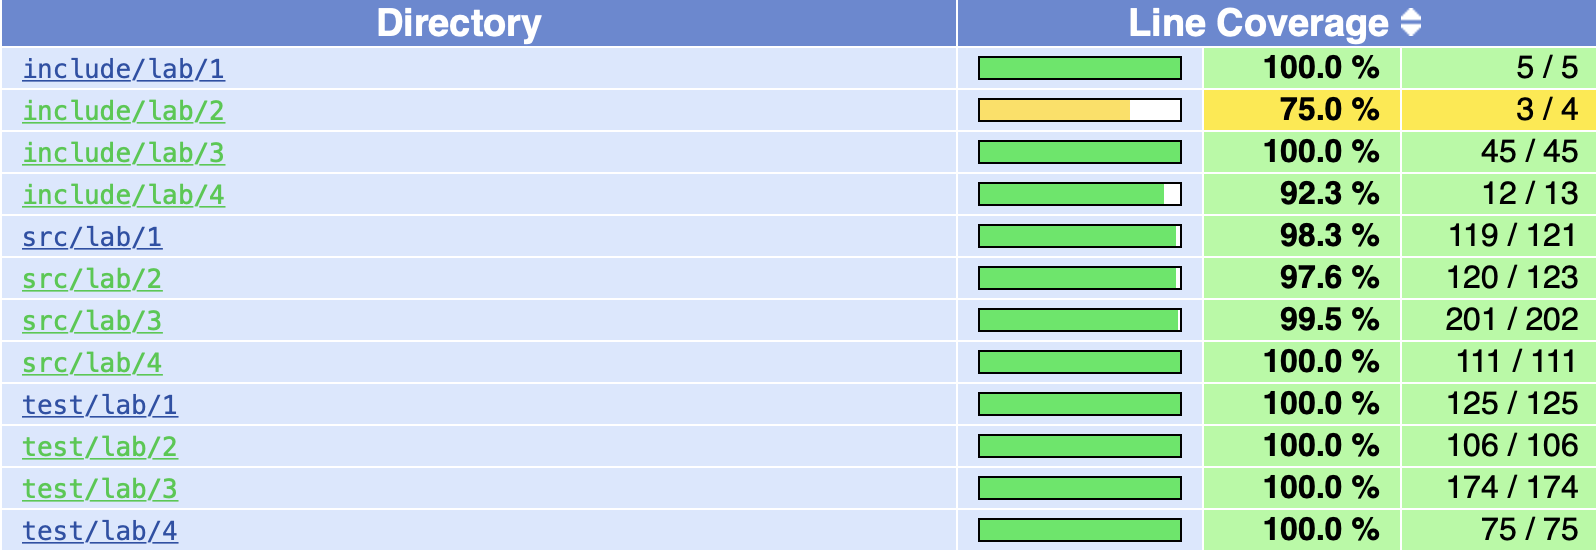
\includegraphics[scale=.5]{cov.png}
\end{figure}

\section{实验结果与分析}\label{sec:test44}
本次实验加深了对图的概念、基本运算的理解,
掌握了图的基本运算的实现。
深刻理解了图的\emph{逻辑结构}和\emph{物理结构}之间的关系。
\par 整个实验均在\texttt{UNIX}环境下编程
所有的代码均采用\emph{Google C/C++}标准代码规范,
通过\texttt{clang-format}和\texttt{clang-tidy}进行格式化和规范化。
\par
同时,在编码过程中,我尽可能地使用了更加现代化的C++代码,例如使用智能指针(\textit{unique\_ptr})来进行资源管理,从而避免了手动管理内存而可能带来的内存泄漏等问题、
例如使用\texttt{auto}关键字来声明函数与变量,从而减少了错误的类型声明或不正确的隐式类型转换。
使得代码可读性更高,更容易维护,更加健壮。这样的规范和编码习惯有助于以后在工作中更高效地完成工作任务。
\par
本系统完整的实现了课程要求的全部功能,并且实现了多图管理和文件存储功能,
系统健壮性良好,可以应对各种情况的输入,且能输出相应的错误提示。
系统测试覆盖度接近100\%,可以认为不会发生逻辑错误
\par

